\chapter{Temporal resolution of photon detection}

In the previous chapter we studied the performance of filters, but we did not
define an algorithm to search for signals. Neither we will do it here, we'll
skip it and measure the temporal localization precision once we know there's a
signal.

To this end, we make a simulation where each ``event'' contains only one signal
at a known position. In principle we could use the LNGS data
(section~\ref{sec:lngsdata}), but we don't know the jitter of the trigger pulse
and we may reach a temporal resolution below the sampling period, while in the
simulation we have the exact actual temporal location of signals.

The code is in the same repository of the previous chapter,
\url{https://bitbucket.org/Gattocrucco/sipmfilter}.

\section{Event generation}

Each event is the sum of a signal and a noise waveform. We don't add a
baseline, so the noise has mean zero and the signals taper down to zero. The
signals are negative. We use the same scale of the LNGS data; it actually does
not matter because we are not simulating digitalization.

\subsection{Signal}
\label{sec:toysignal}

We obtain the signal waveform by averaging single photon pulses from the LNGS
data (see section~\ref{sec:lngsdata} for a description of the dataset). We do
not try to align the signals, assuming that they are aligned relative to the
beginning of each acquisition event. We take 3584 \SI1{GSa/s} samples.
Figure~\ref{fig:toytempl} shows the obtained signal template.

(A study not reported here shows that better alignment is achievable but makes
a small difference, and worse alignment means the peak of the signal is smeared
thus yielding lower performance in signal localization, and so our choice is
irrelevant at best, conservative at worst.)

\begin{figure}
    \hspace{0.00\textwidth}
    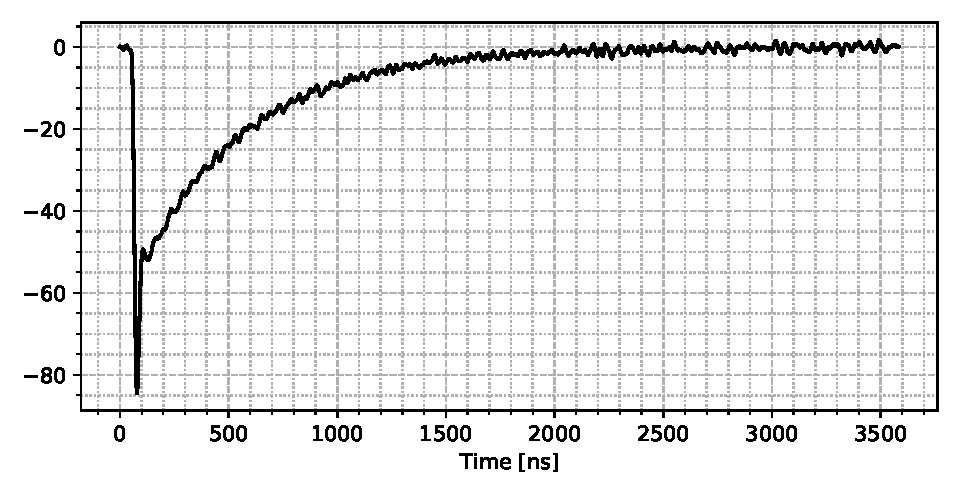
\includegraphics[width=1.00\textwidth]{figtoytempl}
    
    \caption{The source \SI1{GSa/s} signal template used in the simulation.}
    
    \label{fig:toytempl}
\end{figure}

The template is at \SI1{GSa/s}, but the simulation is at \SI{125}{MSa/s}. We
have to downsample the template and shift its temporal position continuously
instead of by $(\SI1{GHz})^{-1} = \SI1{ns}$ steps. Given the continuous
temporal position where we want to place the template, we round it by excess
and defect to the \SI{1}{ns} timebase. Then we downsample the template by
averaging samples in groups of~8, once with the groups aligned to the floor
rounded position, once with the ceiling rounded one. Finally we interpolate
linearly between the two downsampled templates. Figure~\ref{fig:interptempl}
shows a series of waveforms obtained in this way.

(Downsampling with an average is not the best antialiasing filter doable, but
it should be reasonably fine since the higher spectral part is already
suppressed in the signal template.)

\marginpar{I've not said I'm varying the signal amplitude. Maybe I should drop
it from the simulation altogether.}

\begin{figure}
    \hspace{0.00\textwidth}
    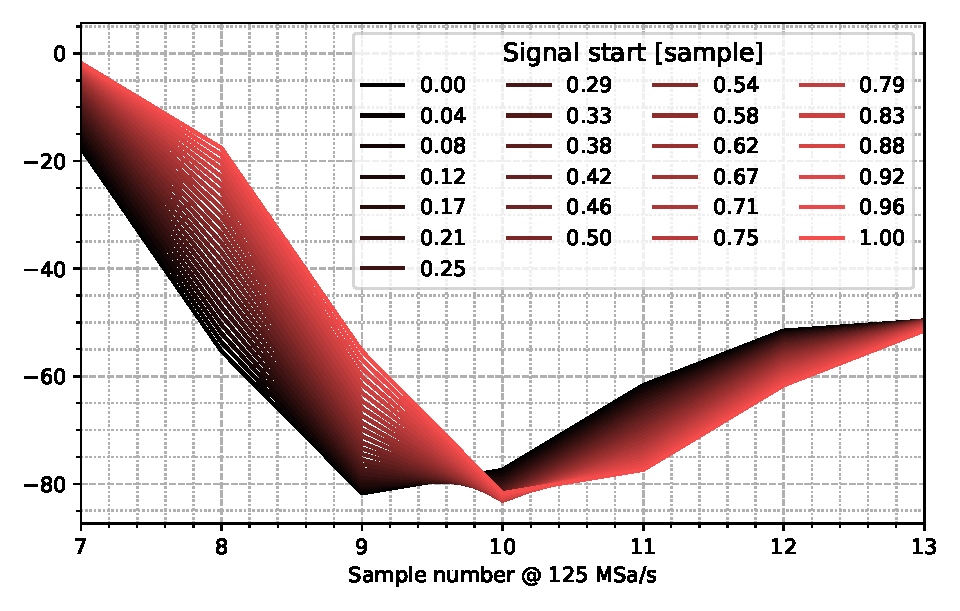
\includegraphics[width=1.00\textwidth]{figinterptempl}

    \caption{The signal template downsampled from \SI1{GSa/s} to
    \SI{125}{MSa/s} and translated continuously instead of by discrete steps
    with linear interpolation.}
    
    \label{fig:interptempl}
\end{figure}

\subsection{Noise}

We used three different kinds of noise: gaussian white noise; noise sampled
from the LNGS data; noise sampled from Proto0 data.

The white noise is generated in the simulation. The LNGS noise is copied from
the same data we used to make the signal template by taking the part of the
events before the signals and filtering out a few events that contained
spurious signals in that location. The Proto0 noise is copied from an
acquisition made on the same PDM when it was used in the Proto0 setup with the
SiPMs under breakdown voltage, thus inactive.

The noise obtained from data is normalized to the variance required by the
simulation. For both LNGS and Proto0 noise the data comes divided in events and
we normalized separately for each event in case the variance changed.

We downsample the noise in the same way as the signal, by averaging nearby
samples. Both noises have spectra that go down with frequency (see
section~\ref{sec:spectrum}), so this crappy antialiasing should be sufficient.
The normalization to the desired variance is done after downsampling. The order
matters because downsampling with averaging reduces the variance of the noise.
See figure~\ref{fig:noise}. The Proto0 noise data is already at \SI{125}{MSa/s}
and so did not require downsampling for most of the simulations.

\begin{figure}
    \hspace{0.00\textwidth}
    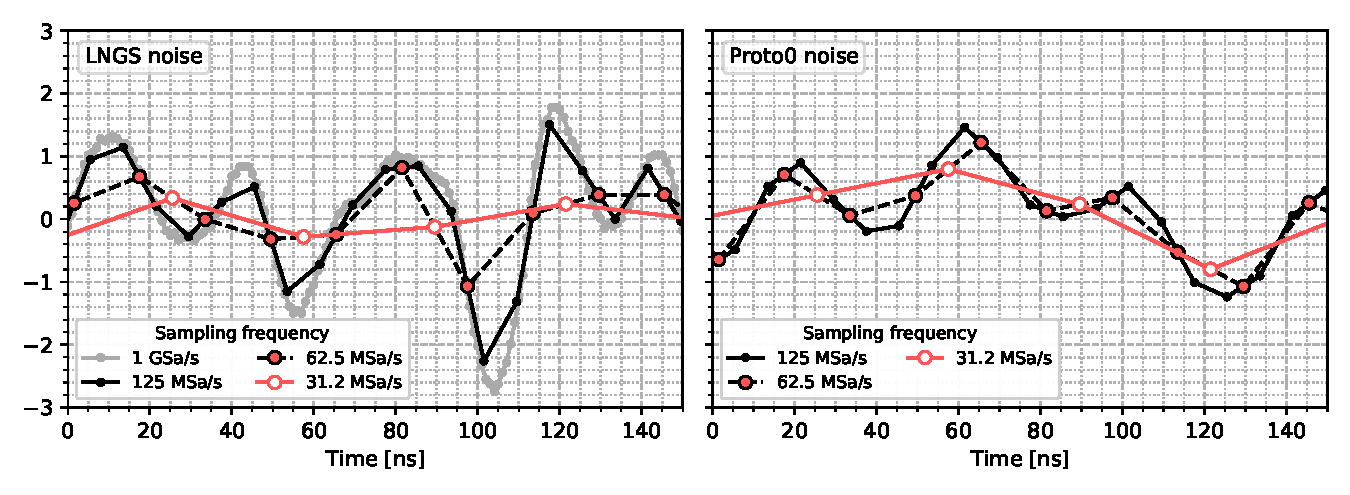
\includegraphics[width=1.00\textwidth]{fignoise}
    
    \caption{The LNGS noise at the original sampling frequency (normalized to
    unit variance) and downsampled.}
    
    \label{fig:noise}
\end{figure}

\subsection{Event layout}

Each event is the sum of a noise waveform and a shorter signal waveform. Before
the beginning of the signal there's a noise-only region long enough for the
filters to be in a stationary state when they reach the signal; in particular
its length is the highest filter length parameter used in the simulation
(\SI{2048}{ns}) plus \SI{256}{ns}.

The simulation is repeated for various signal to noise ratios (SNR). We define
the SNR as follows: the peak height relative to the baseline of the original
\SI1{GSa/s} signal template over the noise standard deviation.

Simulations with different SNR differ only in the multiplicative constant of
the noise, so we used exactly the same noise and signal arrays for each SNR to
speed up the code. This means that there's no random variation between results
obtained at different SNR (or with different filters), keep this in mind when
the smoothness of some plots would seem to suggest that the Monte Carlo error
is negligible.

Figure~\ref{fig:toyevent} shows a complete example event.

\begin{figure}
    \hspace{-0.15\textwidth}
    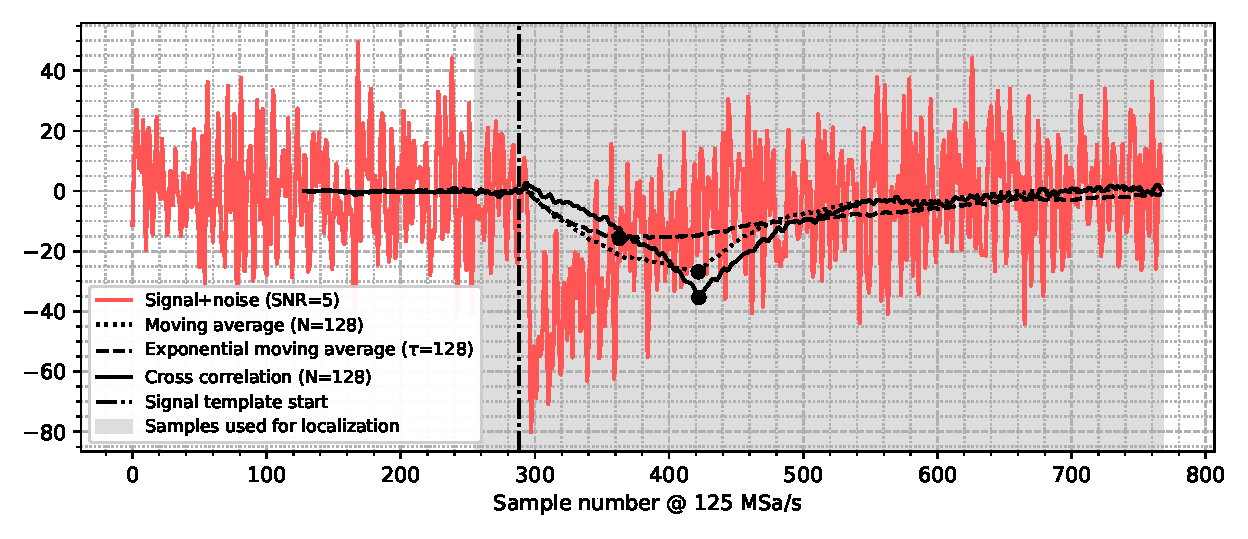
\includegraphics[width=1.30\textwidth]{figtoyevent}
    
    \caption{A simulation event. The dots are the minima of the filters output.
    The minima are searched in the shaded region only; this makes no difference
    with high enough SNR like in this example, but in the limit SNR = 0 the
    minimum fluctuates around uniformly: the search range sets the endpoints of
    this distribution.}
    
    \label{fig:toyevent}
\end{figure}

\section{Temporal localization}

We run the three filters described in section~\ref{sec:filters} (moving
average, exponential moving average, cross correlation), then take the minimum
(the signals are negative) of the filtered waveform as the location of the
signal. We also take the minimum of the unfiltered waveform as baseline
comparison.

The minimum of the filter output occurs in some sense later than the signal
location, this is not a problem since the choice of the point of the signal to
be taken as reference is already arbitrary.

To make the template for the cross correlation filter, we first cut the signal
template (section~\ref{sec:toysignal}) to the required filter length, keeping
the part of the template with maximum euclidean norm, then we downsample it by
averaging nearby samples. See figure~\ref{fig:toyfilttempl}.

\begin{figure}
    \hspace{0.00\textwidth}
    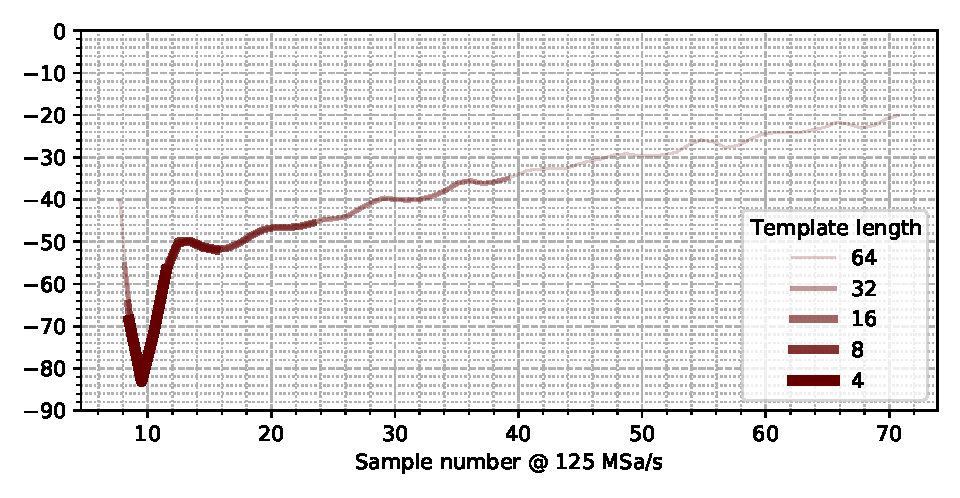
\includegraphics[width=1.00\textwidth]{figtoyfilttempl}
    
    \caption{Some cross correlation filter templates for different lengths. It
    may appear strange that the endpoint on the left has a different height
    than the endpoint on the right for a given template, since we choose the
    truncation to maximize the norm; it happens because we downsample
    \emph{after} truncation.}
    
    \label{fig:toyfilttempl}
\end{figure}

To allow for a localization eventually more precise than the sampling timebase,
we interpolate the minimum sample and its first neighbours with a parabola. We
also try upsampling the waveform to \SI{1}{GSa/s} (with sample repetition)
prior to filtering to check if it improves performance.

\subsection{Resolution}

We repeat the simulation for 1000 events for each filter, filter length
parameter, and SNR in some range, using the Proto0 noise.
Figure~\ref{fig:lochist} shows the histograms of the temporal localization for
all filters for a choice of SNR and filter length.

\marginpar{Specify how the signal template position varies.}

\begin{figure}
    \hspace{-0.07\textwidth}
    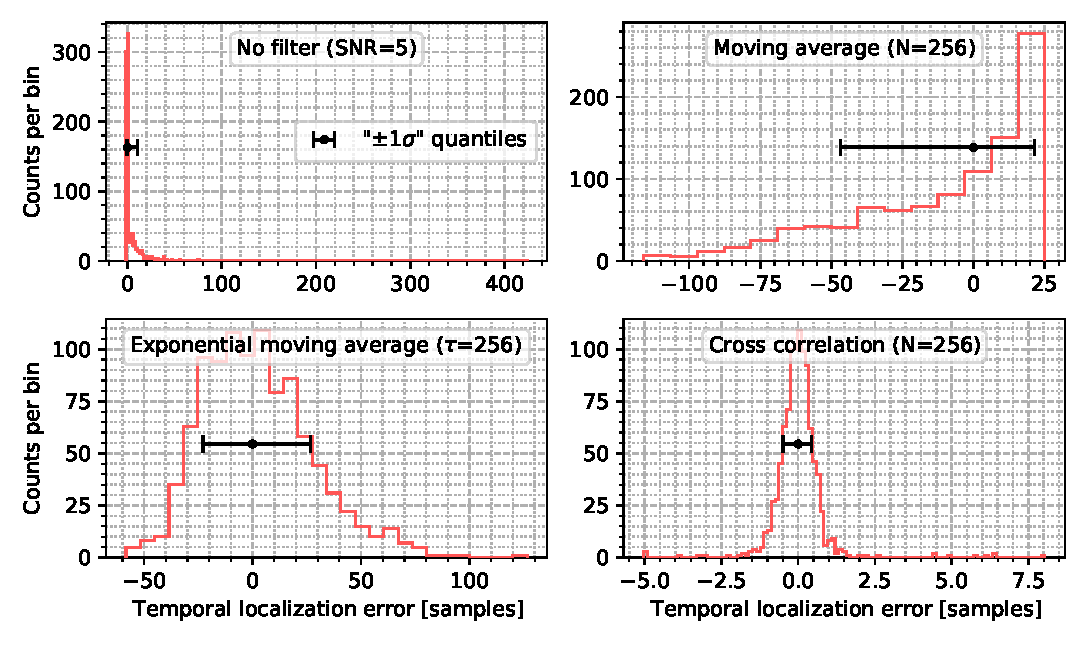
\includegraphics[width=1.13\textwidth]{figlochist}
    
    \caption{Histograms of the temporal localization error, i.e.\ the
    difference between the filter output minimum and the signal template start,
    translated to have zero median, for a choice of SNR and filters length. The
    error bars mark the \SI{16}\% and the \SI{84}\% quantiles. As definition of
    temporal resolution we take half the distance between those quantiles.
    The sampling step is \SI{8}{ns}.}
    
    \label{fig:lochist}
\end{figure}

We see that the distribution of localizations can be non-gaussian, so to
quantify the resolution we use, instead of the standard deviation, half the
distance between the \SI{16}\% and \SI{84}\% quantiles, which is equivalent to
a standard deviation for a gaussian, but gives a meaningful measure for the
width of the distribution even when it's highly skewed or with heavy tails.

Figure~\ref{fig:rescurve} shows the temporal resolution thus defined for each
filter, filter length, and SNR. The exponential moving average has a
consistently poor performance compared to the other filters. The
cross-correlation filter is the best one, with performance improving with
length, and at a length of 96 samples (\SI{512}{ns}) is already practically
optimal. The moving average can get close to the cross-correlation filter by
choosing appropriately the number of samples.

\begin{figure}
    \hspace{-0.09\textwidth}
    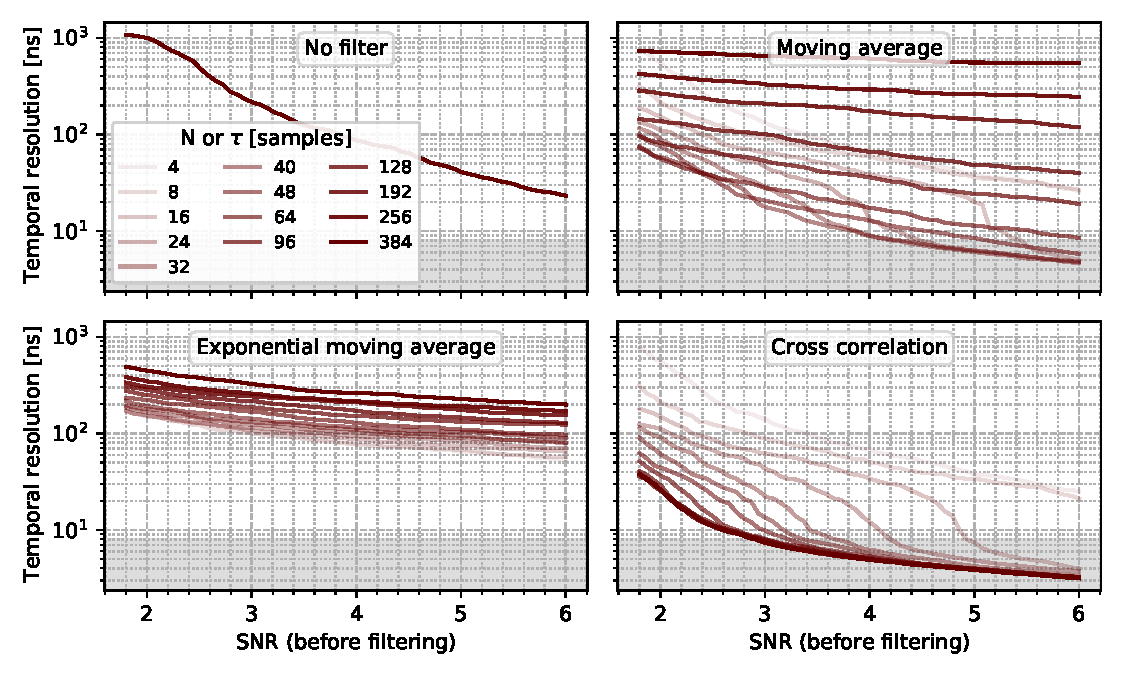
\includegraphics[width=1.17\textwidth]{figrescurve}
    
    \caption{Photodetection temporal resolution for a range of SNR and filter
    lengths. The shaded region marks the sampling step (\SI{8}{ns}). The right
    endpoint of the cross correlation filter curves is at \SI{3}{ns}.}
    
    \label{fig:rescurve}
\end{figure}

The online processing of the PDM output in the experiment will be done in two
steps: the digitizers must find the signals, then send them to the front end
processors (FEPs) for further analysis. The computational resources of the
digitizers are limited compared to the FEPs.

\marginpar{A schematic of the DAQ would be appropriate. Maybe in a previous
introductory chapter.}

The exponential moving average can be surely implemented on the digitizers. The
cross-correlation with 64 samples could probably be done on the digitizers
since a similar computation was implemented in another study.

The FEPs can and should probably use the best filter, so they would run a long
cross-correlation filter. The temporal resolution matters in the FEPs but
probably not in the digitizers, in the latter case it is just a generic measure
of perfomance.

Thus out of all the temporal resolution curves the ones that matter are:
%
\begin{itemize}
    %
    \item the best we can do with the exponential moving average and moving
    average;
    %
    \item the long cross-correlation filters;
    %
    \item the 64 samples cross-correlation filter.
    %
\end{itemize}
%
We plotted these curves together in figure~\ref{fig:rescomp}, adding some
curves done with the LNGS and white noises. Note that a different noise
spectrum makes a large difference at low SNR. We also plot a curve computed
with upsampling; it does not improve significantly the performance.

\begin{figure}
    \hspace{0.00\textwidth}
    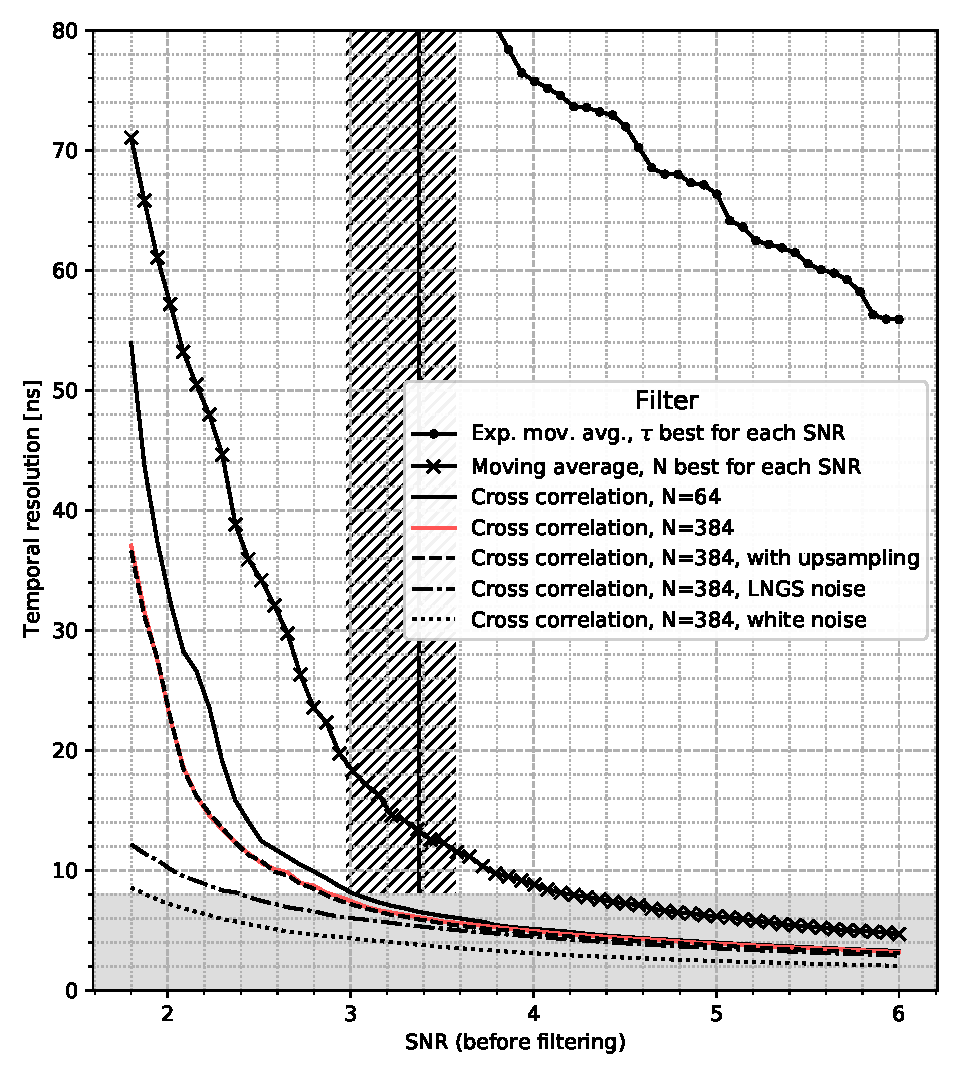
\includegraphics[width=1.00\textwidth]{figrescomp}
    
    \caption{Photodetection temporal resolution vs. SNR for various filters.
    The shaded region marks the sampling step (\SI{8}{ns}). The hatched band is
    the interval of SNR observed in Proto0; the vertical line is the SNR in the
    LNGS data (after downsampling to \SI{125}{MSa/s}). Where not specified, the
    noise is from Proto0.}
    
    \label{fig:rescomp}
\end{figure}

\section{Data reduction}

We said that the digitizers must find signals in the waveform stream and send
them to the FEPs for further processing. The bandwidth of the connection
between the digitizers and the FEPs happens to be a bottleneck. Two possible
ways of reducing the amount of transmitted data are keeping only the minimum
number of samples for each signals, and reducing the sampling frequency. Both
have an effect on the temporal resolution, which we assess here.

\subsection{Waveform truncation}

We repeat the simulation, but this time we use only a fixed smaller number of
samples in each event to compute the filter output. We call this selection of
samples ``window''. On the window we run only a long cross-correlation filter
since that's what would be done on the FEPs. As past and future boundary
condition we use zero. We evaluate the filter even after the sample window end
because the window can be shorter than the filter.

While the length of the window is fixed, the placement is not fixed relative to
the true signal location. Instead we use the temporal localization with another
filter feasible on the digitizers, calibrated to have the median aligned to the
beginning of the signal template. The window then extends a given number of
samples to the left and to the right of this localization.

Figure~\ref{fig:windowevent} shows this procedure graphically for a single
event. Figure~\ref{fig:windowtempres} shows the temporal resolution versus
unfiltered SNR curves for various choices of window length, noise, and filter
used to align the window, where for reasons of computation time the latter was
computed at a fixed SNR that does not follow the value on the x-axis.

\begin{figure}
    \hspace{-0.20\textwidth}
    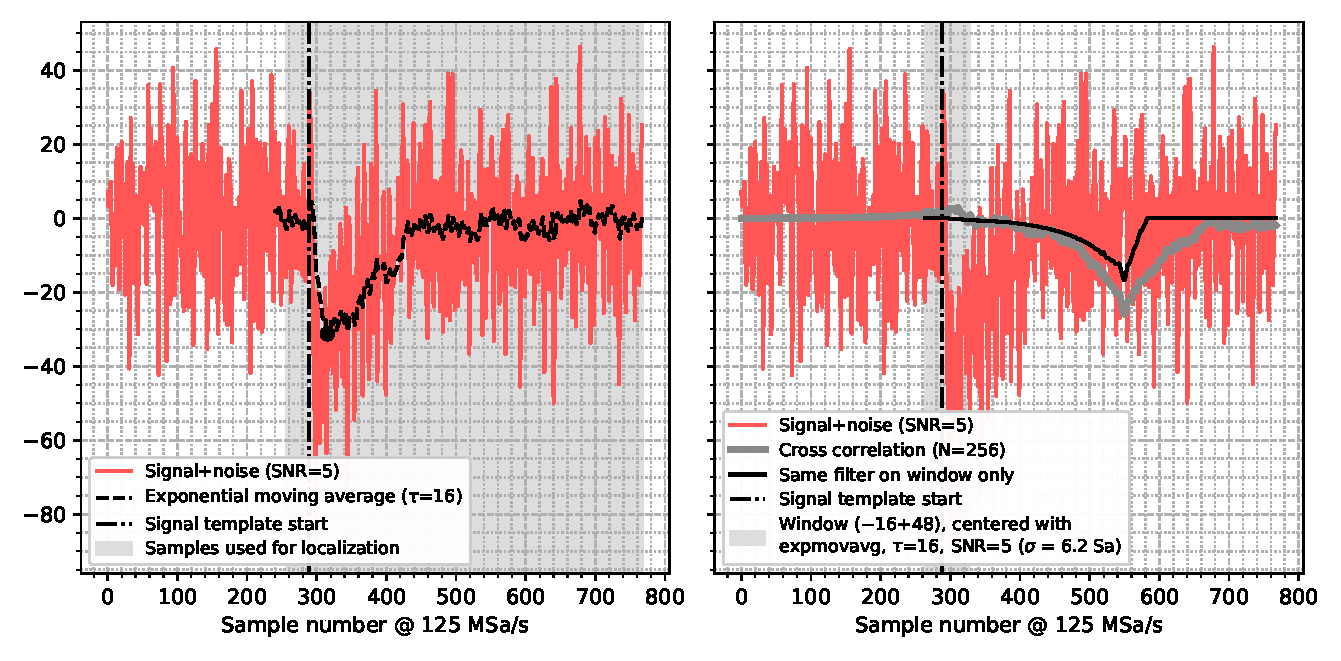
\includegraphics[width=1.40\textwidth]{figwindowevent}
    
    \caption{Left panel: a simulation event filtered with the exponential
    moving average. Right panel: the same event filtered with a long cross
    correlation filter, both using the whole waveform and using only the
    samples in the shaded window, which is centered using the localization from
    the filter in the left panel.}
    
    \label{fig:windowevent}
\end{figure}

\begin{figure}
    \hspace{-0.14\textwidth}
    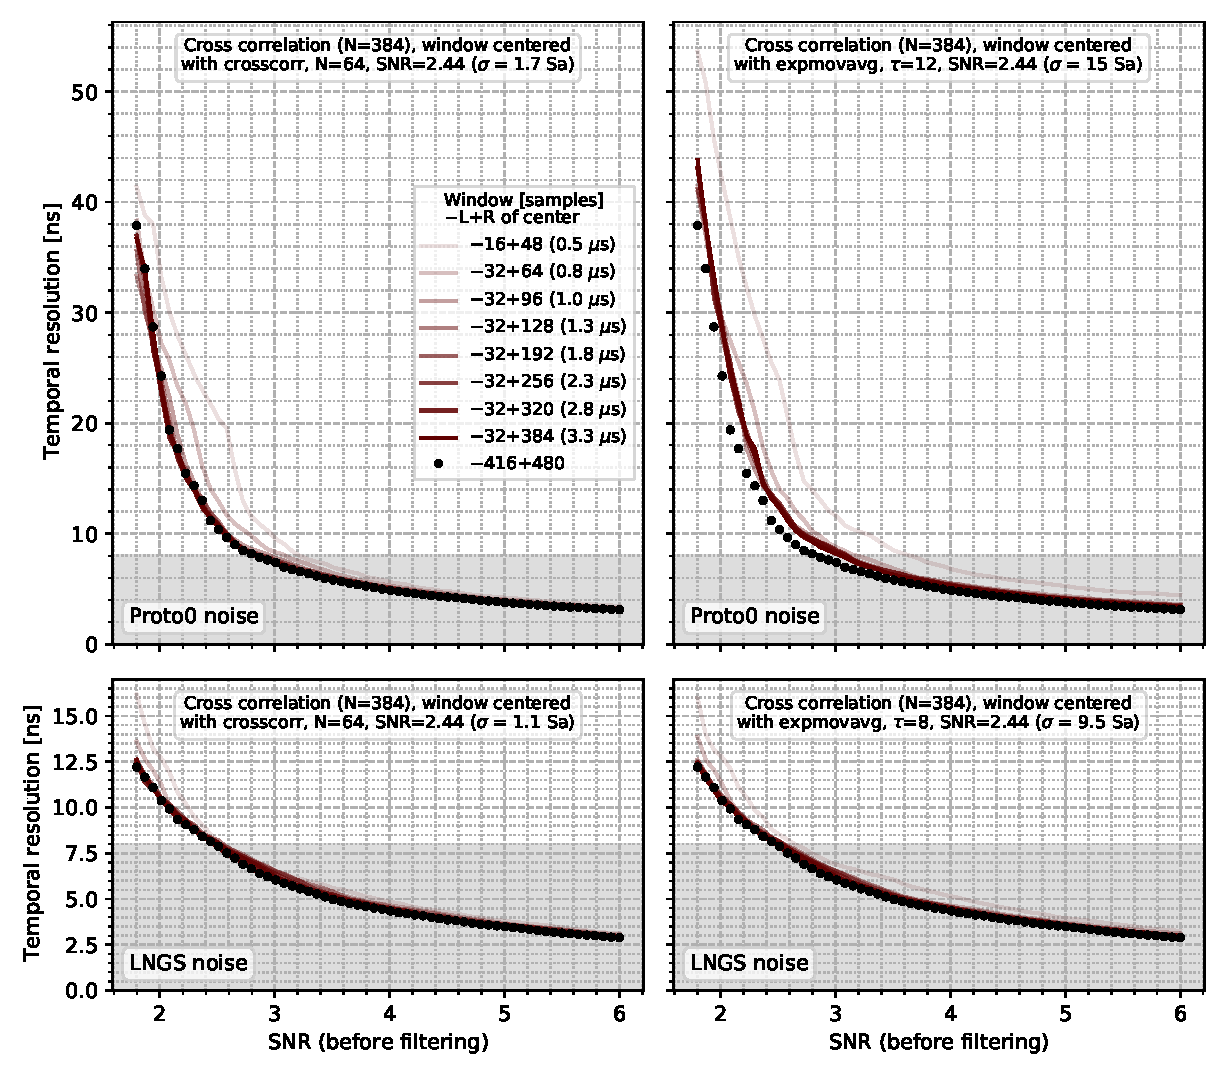
\includegraphics[width=1.28\textwidth]{figwindowtempres}
    
    \caption{Photodetection temporal resolution with a long cross correlation
    filter applied only on a short window of samples centered using a shorter
    cross correlation filter (left panels) or an exponential moving average
    (right panels). The various curves correspond to different window lengths,
    while the black dots are the resolution without windowing.}
    
    \label{fig:windowtempres}
\end{figure}

By looking at figure~\ref{fig:windowtempres}, we conclude that probably it is
sufficient to save \SI1{\micro s} of waveform to obtain practically the same
temporal resolution achievable without windowing.

What's missing in this study is that we did not try to optimize the left/right
balance of the window, and that as said above the unwindowed localization used
to align the windows is done at a mismatched SNR. The first problem can only
worsen the temporal resolution obtained, so it is conservative; the second is
conservative assuming that our choice of SNR (2.4) is lower that what we expect
in the detector.

\marginpar{Maybe with the channel summing this SNR will become realistic.}

\subsection{Downsampling}

Another way of reducing the data throughput is downsampling. In
figure~\ref{fig:tempresdowns} we show the temporal resolution achieved with a
long cross correlation filter, for white and LNGS noise, at different sampling
frequencies. We can observe that downsampling by a factor of 2 from
\SI{125}{MSa/s} to \SI{62}{MSa/s} maintains almost the same temporal
resolution, while going to \SI{31}{MSa/s} lowers it visibly.

\marginpar{Explain the SNR rescaling.}

\begin{figure}
    \hspace{-0.22\textwidth}
    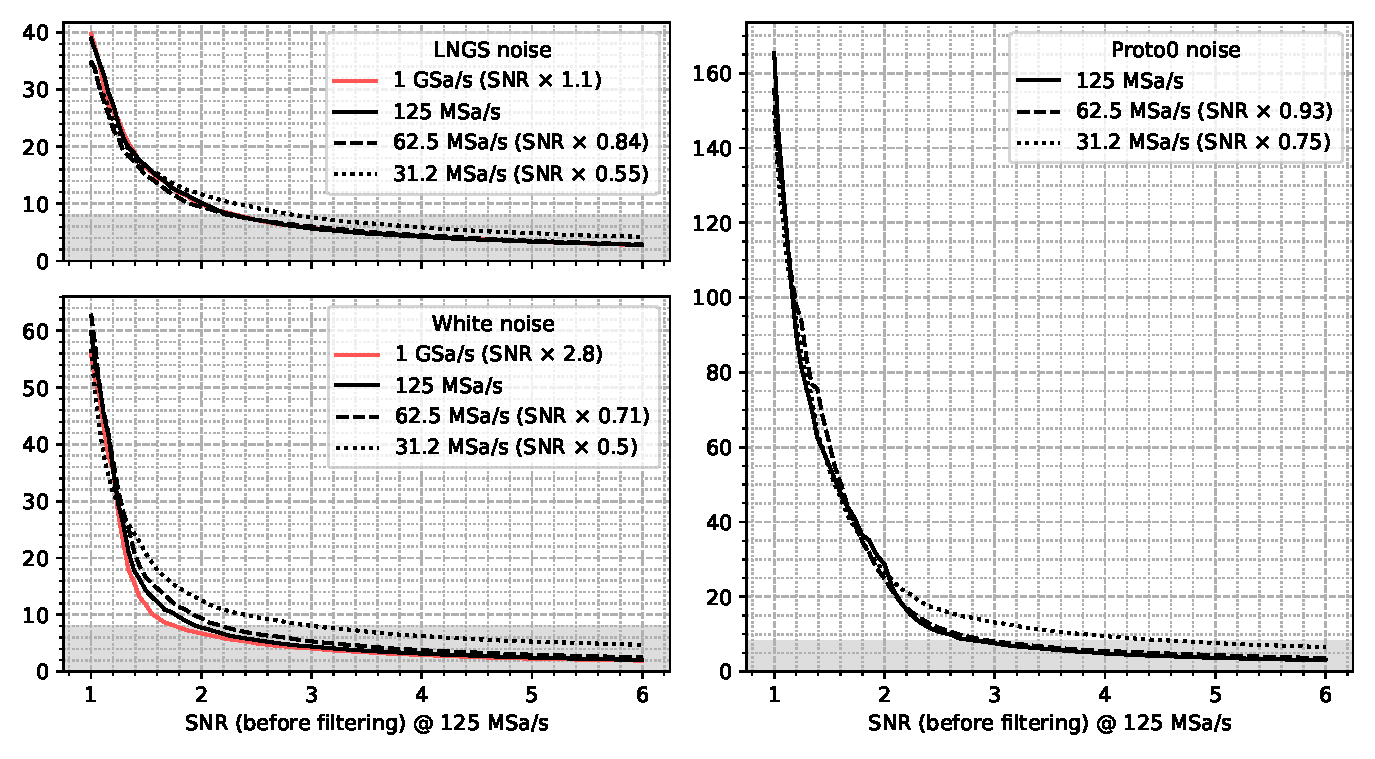
\includegraphics[width=1.43\textwidth]{figtempresdowns}
    
    \caption{Photodetection temporal resolution at different sampling
    frequencies with a cross correlation filter with template length
    \SI{2048}{ns}. The SNR scale is at \SI{125}{MSa/s}; curves for different
    sampling frequencies are rescaled horizontally by the factor written in the
    legend to account for the noise variance reduction with downsampling.}
    
    \label{fig:tempresdowns}
\end{figure}

Since we are downsampling we also need to check if we lose signal to noise
ratio in the filter output. In table~\ref{tab:filtsnrdowns} we report the
ratio between SNR after and before filtering. It does not change significantly
with downsampling.

\begin{table}
    \centering
    \begin{tabular}{c|cccc}
               & \SI{1}{GSa/s} & \SI{125}{MSa/s} & \SI{62.5}{MSa/s} & \SI{31.2}{MSa/s} \\ \hline
        Proto0 &               &             3.6 &              3.6 &              3.6 \\
          LNGS &           6.3 &             6.3 &              6.5 &              6.6 \\
         White &           4.7 &             4.7 &              4.7 &              4.7
    \end{tabular}
    
    \caption{Ratio of SNR after over before filtering. The \SI{125}{MSa/s}
    column contains the actual SNR ratios of the simulations, while the values
    for the other sampling frequencies are divided by the noise standard
    deviation reduction with downsampling relative to \SI{125}{MSa/s} to make
    them comparable.}
    
    \label{tab:filtsnrdowns}
\end{table}
